\chapter{Background}
\section{Handover}
Handover is a crucial technique in radio communication networks for both mobility management and load balancing. Handover is the process in which an active cell connection (data or cellular) is transferred from a source base station to a target station. This is done for multiple reasons, though its core function is to maintain continuous connectivity for mobile devices.
\ab{Explain first what is handover, then why it is used for mobility management and load balancing, so first phrase at the end.}

As a UE (User Equipment - any device which can connect to a cell network, for instance a mobile phone) moves further from a base station (such as a radio tower) the signal strength decreases with a function of distance (propagation loss), as well as line of sight (LOS) considerations. We measure signal strength using Received Signal Reference Power (RSRP) as reported by the UE. 5G and new radio (NR) use much higher frequency for data transmission, especially mmWave technology. High frequencies suffer from much higher propagation loss, and have a much higher LOS dependency due to the inability to penetrate obstacles. For this reason, 5G base stations cover a much small range, termed their "cell", and 5G cells therefore are much denser. This leads to a much higher number of handovers occurring.
\ab{Explain first how handover is executed. It is based on the RSRP and when the RSRP from the target base station is better than from the source base station, handover is triggered by the source base station.}

\ab{The main motivation is that handover is simple in outdoor environments, but 5G will be ubiquitously deployed in indoor environments. The wireless indoor channel is much harder to model as sudden changes of the RSRP due to obstacles might trigger unnecessary handovers if the obstacles disappear as the UE is moving. Hence the main motivation is to understand and predict handover in indoor environments.  }

This leads into the motivation for this paper, as connection drops, and reduced throughput due to handovers have a much greater impact on the overall Quality-of-Service (QoS) for UEs. In this paper, we explore the associated challenges in optimising handover, both in terms of mobility management, as well as load balancing.

\section{Challenges}
\subsection{Mobility Management}
Mobility Management is an integral part of a cellular network, and ensures UEs maintain a good quality connection to the network. UEs, as mobile devices, do not remain stationary, and will move through different cells as a person walks, moves or drives. The Mobility Management Unit (MMU) will transfer the connection of the device between different station through the use of handover. As and when to initiate handover is a very broad topic with hundreds of research papers dedicated to optimising various parameters and metrics, and is not a simple decision. Premature handover can lead to a phenomenon termed Handover Ping Pong (HOPP) where a UE is transferred back to the source cell in a short period of time, thereby having needlessly interrupted the UEs cell connection twice, as well as increasing the server load. Late handover can lead to a cell experiencing much lower data throughput, or disconnecting entirely from the network (Handover Failure, HOF).

A key difficulty therefore can come from fast-moving users, as handovers must be performed much faster.

\subsection{Load Balancing}
Another key factor to consider is Load Balancing in a cellular network. Active cell connections require a certain amount of hardware resources, and therefore to maintain good performance across the network, handovers should not just be employed for mobility management, but also for equitable distribution of traffic across base stations. This ensures efficient resource utilisation and reduces congestion. A careful balance must be struck to offset individual UE performance with average network performance using handovers.

\section{Handover Algorithms}
The focus of this paper is to understand the effects of handover, and to design and test various strategies to minimise the negative effects. We therefore need to understand the various methods used to initiate handover, and classify the various algorithms. An important distinction to note is that while the \textit{UE} provides the measurement reports \ab{explain firstly what the measurement report is}, \st{it is} the base station \st{which} will decide to initiate handover based on the report.
\subsection{Classical Approach}

The standard approach taken towards handover \st{is to} uses two parameters, \textit{Hysteresis} and \textit{Time to Trigger}, to determine when to trigger handover. When a neighbor cell has an RSRP greater than the current cell by a set margin, \ab{i.e.,} the hysteresis, for a given period of time, \ab{i.e.,} time to trigger\st{,}. \st{Then a handover is initiated} \ab{The handover is triggered and the UE is transferred to the neighbor cell}. This process is illustrated in Figure \ref{fig:hysteresis_handover}. Alternative heuristics are often needed, \st{as hysteresis and time to trigger} \ab{as the standard approach is not robust enough for dynamic environments.} \st{creates a fairly rigid algorithm, one which is not flexible to dynamic environments}.

\begin{wrapfigure}[18]{r}{0.5\textwidth}
    % \centering
    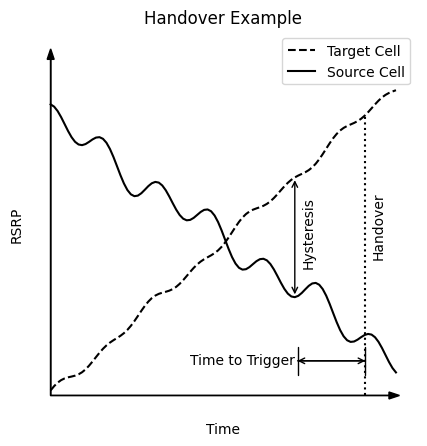
\includegraphics[width=0.48\textwidth]{hysteresis_ttt.png}
    \caption{Handover based on Hysteresis and TTT}
    \label{fig:hysteresis_handover}
\end{wrapfigure}

% \clearpage %============================= CLEAR PAGE  =====================================%

\subsection{Alternative Heuristics}
The Hysteresis and TTT \ab{TTT is the first time to appear and I do not know which is the meaning} form the basis of the majority of existing handover algorithms but are by no means the only parameters used. Other possible parameters used in the literature are throughput, location, load balancing, user’s velocity, service delay, and distance. \cite{nyangaresi_efficient_2022}. \ab{Explain how these parameters are used for handover}

\subsection{Machine Learning}
Seeing handover as an optimisation problem, the utilisation of Machine Learning \ab{include the acronym Machine Learning (ML)} into the problem of handover is a natural one. For this reason, \st{there is a great emphasis on current literature on the feasibility of using different ML techniques in comparison to more naive algorithms} \ab{ML techniques are appealing to provide better performance than the more naive algorithms.}

ML algorithms can be subdivided into supervised, unsupervised and reinforcement learning. Supervised and unsupervised algorithms perform either regression or classification on a set of inputs. Our problem, however, deals with learning the optimal policy \ab{explain what the optinmal poloicy is}, \st{and for that reason} \ab{therefore} reinforcement learning is most often used. Reinforcement learning is based on the concept that the algorithm will learn to maximise its rewards in a given environment by learning the optimal policy. For us, this can be formulated as the algorithm maximising RSRP, throughput or quality of service, whilst minimising high loads, through initiating handovers. This has been explored in many recent papers as surveyed in \citet{mollel_survey_2021}.

\citet{mollel_survey_2021} introduces and surveys an alternative method of using machine learning. The pure network-based models operate only on radio data, such as RSRP and base station states, however, an alternative heuristic \st{is to} use\ab{s} optical information, such as camera feeds to better predict handover. This is done through tracking UE movement through object detection, and predicting when LOS will be obstructed. While this is a tool that can prove very useful, it introduces many limitations as the models trained will be very location dependant, and has the greatest impact in indoor 5G mmWave networks due to the LOS dependency.

\section{Handover Testbeds}
To evaluate experimental algorithms, we need some way to emulate a network. Many authors choose to run custom simulations using propagation algorithms to model path loss, and simulate the network devices. A much better method is to use a software radio suite as a \st{test bed} \ab{testbed}. This allows \st{us} to emulate UEs, base stations (BSs), and the core network \ab{in real scenarios}(CN)\st{, with the radio connections between devices simulated by GNUradio}.

There are a few options available for use, with the major software's being srsRAN, OpenAirInterface and Aether. For this paper, srsRAN is chosen due to its clear open source code, and extensive tutorials to get started with. While a fully custom testbed allows for greater flexibility, the realistic nature of using software radio suites will give results which much better reflect how the algorithms would perform in a real world scenario, and so arguably given more useful results.


\section{Previous Work}

\ab{Include papers that model and/or measure the negative impact of handover in indoor scenarios, whether is simulation or real-world analysis.}

\citet{hatipoglu_handover-based_2020} The paper presented a handover-based load balancing algorithm for HetNets. The paper utilised UE speeds in determining handover, an metric which is unrealistic to obtain in practice. The algorithm itself is fairly simplistic, and while the paper showed good results, the algorithm does not consider key metrics such as RSRP, or connection speed.
 
\citet{powell_handover_2021} The paper presented a testing framework for 4G experiments using srsRAN, and performed basic experiments with it. The framework was presented clearly, and I was able to replicate the results of their simulation. The experiments they performed however were limited as signal strength was arbitrarily introduced by attenuating a signal, and did not utilise signal propagation algorithms.

\citet{yajnanarayana_5g_2020} The paper presented a handover algorithm using Contextual Multi-Armed Bandit reinforcement learning. This ML model provided modest improvements (0.3dB) in average RSRP of devices. The authors also wrote their own network simulator, one which used sophisticated propagation models, such as log-shadowing, as well as the WINNER UMa Model. The code used to simulate it was not released however, providing very little reproducability of the paper. The improvements were also not very large, and better results could possibly be obtained with a deep learning based Reinforcement model

\section{Research Gap}
\begin{itemize}
    \item Load Balancing in realistic testbed
    \item Improve LB with better heuristics
\end{itemize}

\section{Other points}
\begin{itemize}
    \item Reactive vs Predictive
    \item Use SINR for HO params
    \item Spikes in traffic due to events, past data
    \item Colloseun Emulator
    \item O-RAN
\end{itemize}